
\documentclass[preprint,12pt]{elsarticle}

\usepackage[spanish]{babel}
\usepackage{amssymb}
\usepackage{graphicx}
\usepackage{lineno}
\usepackage[utf8]{inputenc}
\usepackage{url}
\usepackage{natbib} 
\usepackage{amsmath} 
\usepackage{amssymb} 
\usepackage{float}

\begin{document}
	
	\begin{frontmatter} 

		\title{\huge Instalación de un Gestor de Base de Datos Oracle INFORME DE LABORATORIO 08 }
		
		\author{Pacora Silva Jorge Carlos         	(2013000725)} 
		\address{Escuela Profesional de Ingeniería de Sistemas}
		\address{Universidad Privada de Tacna}
		\address{Tacna, Perú}
	\end{frontmatter}



\section{INFORMACIÓN GENERAL} 

\subsection {\textbf{Objetivos}}
\begin{itemize}
	\item Instalación de OracleDatabase en Docker
	\item Usar docker con  Oracle SQL Developer for Windows
\end{itemize}

\subsection {\textbf{Equipos, materiales, programas y recursos utilizados}}
\begin{itemize}
	\item Computadora con sistema operativo Windows XP, Vista, Windows 7, Windows 8 y/o Windows 8.1.
	\item Virtualization activada en el BIOS..
	\item CPU SLAT-capable feature
	\item Al menos 4GB de RAM.
	\item Docker Desktop 
	\item Oracle SQL Developer for Windows
\end{itemize}


\section{Marco Teórico}


\subsection {\textbf{Docker}}
Docker es un proyecto de código abierto que automatiza el despliegue de aplicaciones dentro de contenedores de software, proporcionando una capa adicional de abstracción y automatización de virtualización de aplicaciones en múltiples sistemas operativos.
\subsection {\textbf{Contenedores}}
Un contenedor es más ligero, ya que mientras que a una máquina virtual necesitas instalarle un sistema operativo para funcionar, un contenedor de Docker funciona utilizando el sistema operativo que tiene la máquina en la que se ejecuta el contenedor.
\subsection{\textbf{Oracle SQL Developer}}
Oracle SQL Developer es un entorno de desarrollo integrado para trabajar con SQL en bases de datos Oracle. Oracle Corporation ofrece este producto gratis; utiliza el kit de desarrollo de Java.


\section{PROCEDIMIENTO}

\subsubsection{\textbf{Paso 1: Verificar la disponibilidad de Docker}}
\begin{figure}[H]
	\begin{center}
		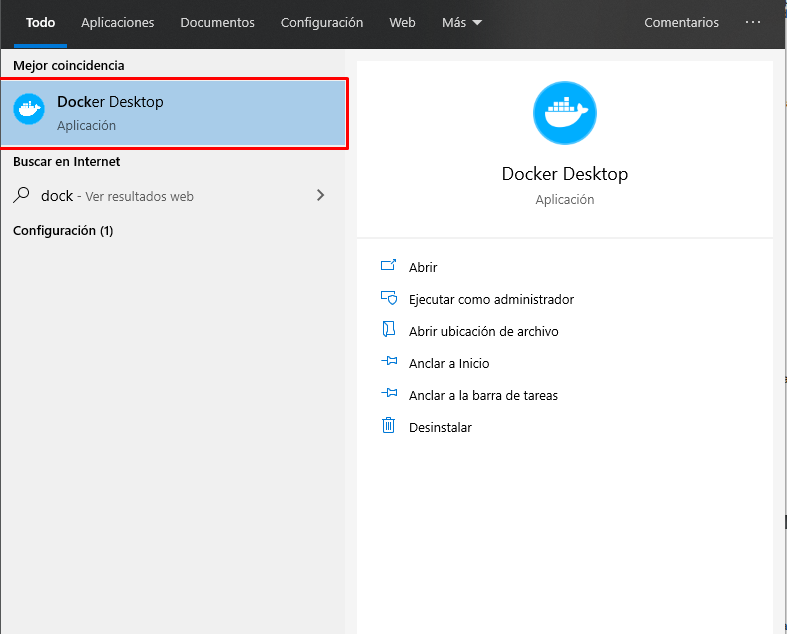
\includegraphics[width=12cm]{./IMAGENES/foto1} 
		\caption{Vizualizar Docker Setup}
	\end{center}
\end{figure}
\begin{figure}[H]
	\begin{center}
		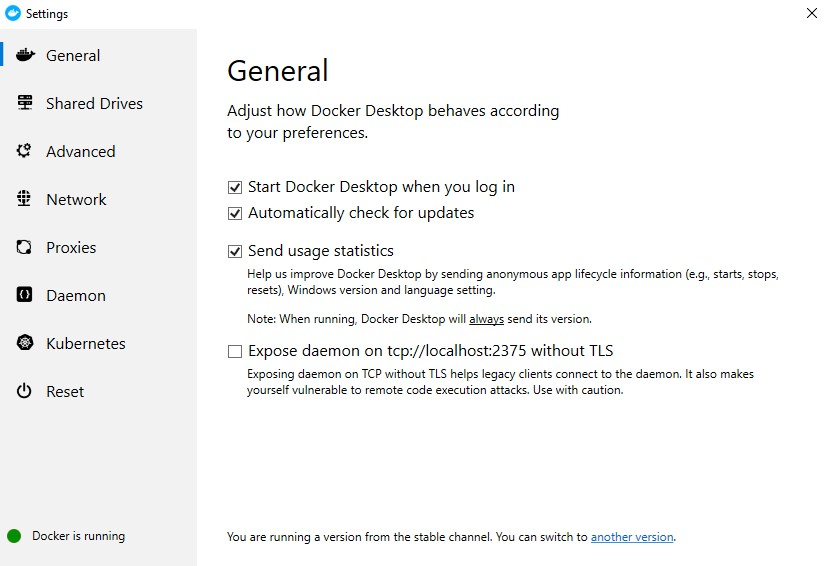
\includegraphics[width=12cm]{./IMAGENES/foto4} 
		\caption{Mostrando el menu de docker}
	\end{center}
\end{figure}

\subsubsection{\textbf{Paso 2: Usando los Comandos en Docker}}

\begin{figure}[H]
	\begin{center}
		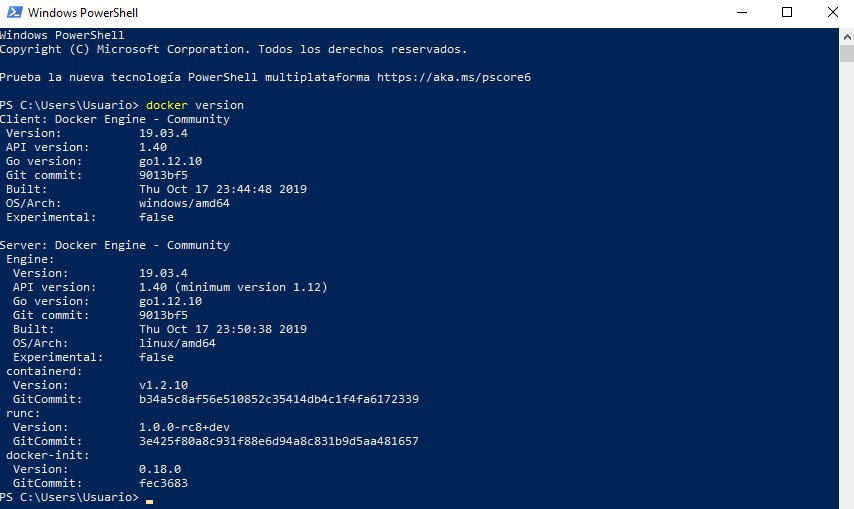
\includegraphics[width=12cm]{./IMAGENES/foto5} 
		\caption{Docker version que nos mostrara algunas especificaciones}
	\end{center}
\end{figure}


\begin{figure}[H]
	\begin{center}
		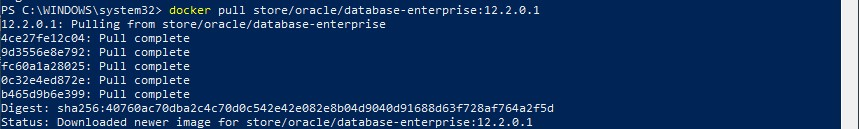
\includegraphics[width=12cm]{./IMAGENES/imagen2} 
		\caption{Lo cual descargará la imagen del contenedor de Oracle Database en un servidor Linux}
	\end{center}
\end{figure}

\begin{figure}[H]
	\begin{center}
		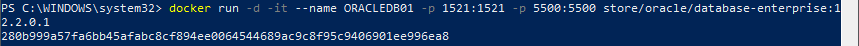
\includegraphics[width=12cm]{./IMAGENES/IMAGEN3} 
		\caption{comando para correr docker en un puerto}
	\end{center}
\end{figure}
\begin{figure}[H]
	\begin{center}
		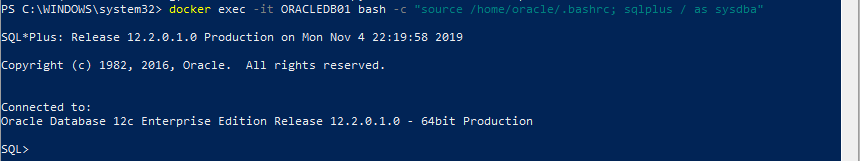
\includegraphics[width=12cm]{./IMAGENES/IMAGEN5} 
		\caption{Executar docker con ORACLE}
	\end{center}
\end{figure}

\begin{figure}[H]
	\begin{center}
		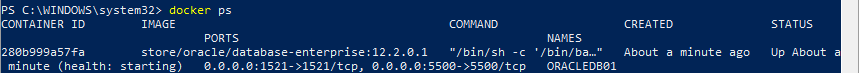
\includegraphics[width=12cm]{./IMAGENES/IMAGEN4} 
		\caption{ORACLE INSTALADO}
	\end{center}
\end{figure}

\begin{figure}[H]
	\begin{center}
		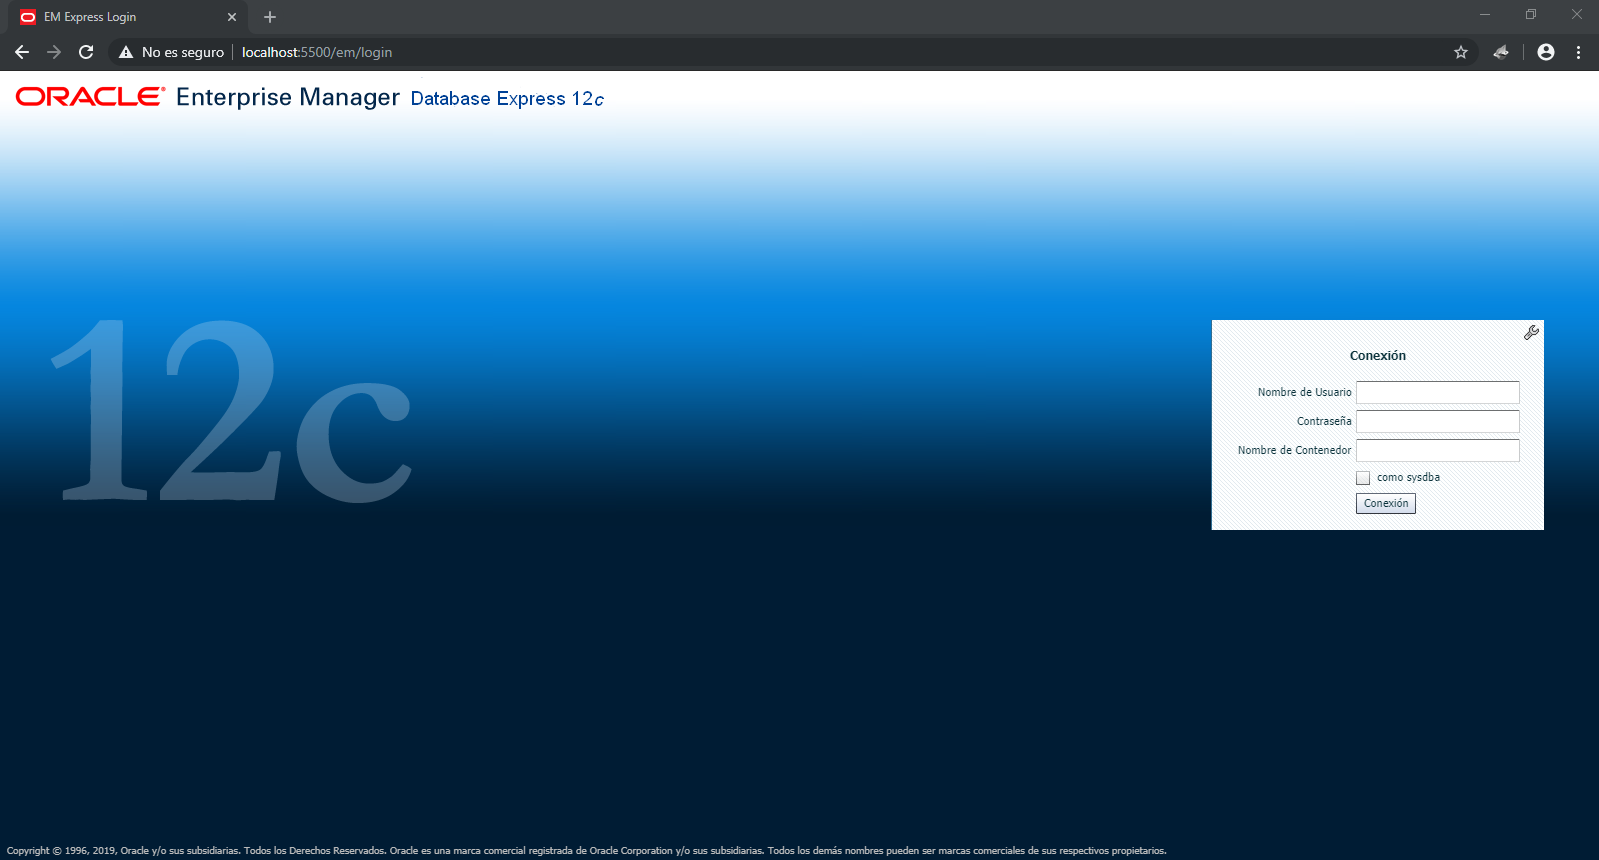
\includegraphics[width=12cm]{./IMAGENES/IMAGEN7} 
		\caption{Abriendo ORACLE CON LOCALHOST}
	\end{center}
\end{figure}

\subsubsection{\textbf{Paso 3: Oracle SQL Developer}}
\begin{figure}[H]
	\begin{center}
		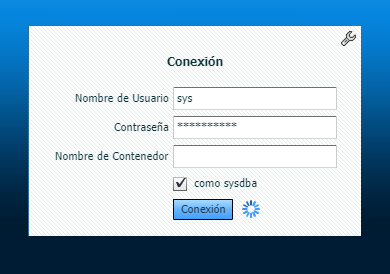
\includegraphics[width=12cm]{./IMAGENES/IMAGEN8} 
		\caption{Ingresamos al login}
	\end{center}
\end{figure}

\begin{figure}[H]
	\begin{center}
		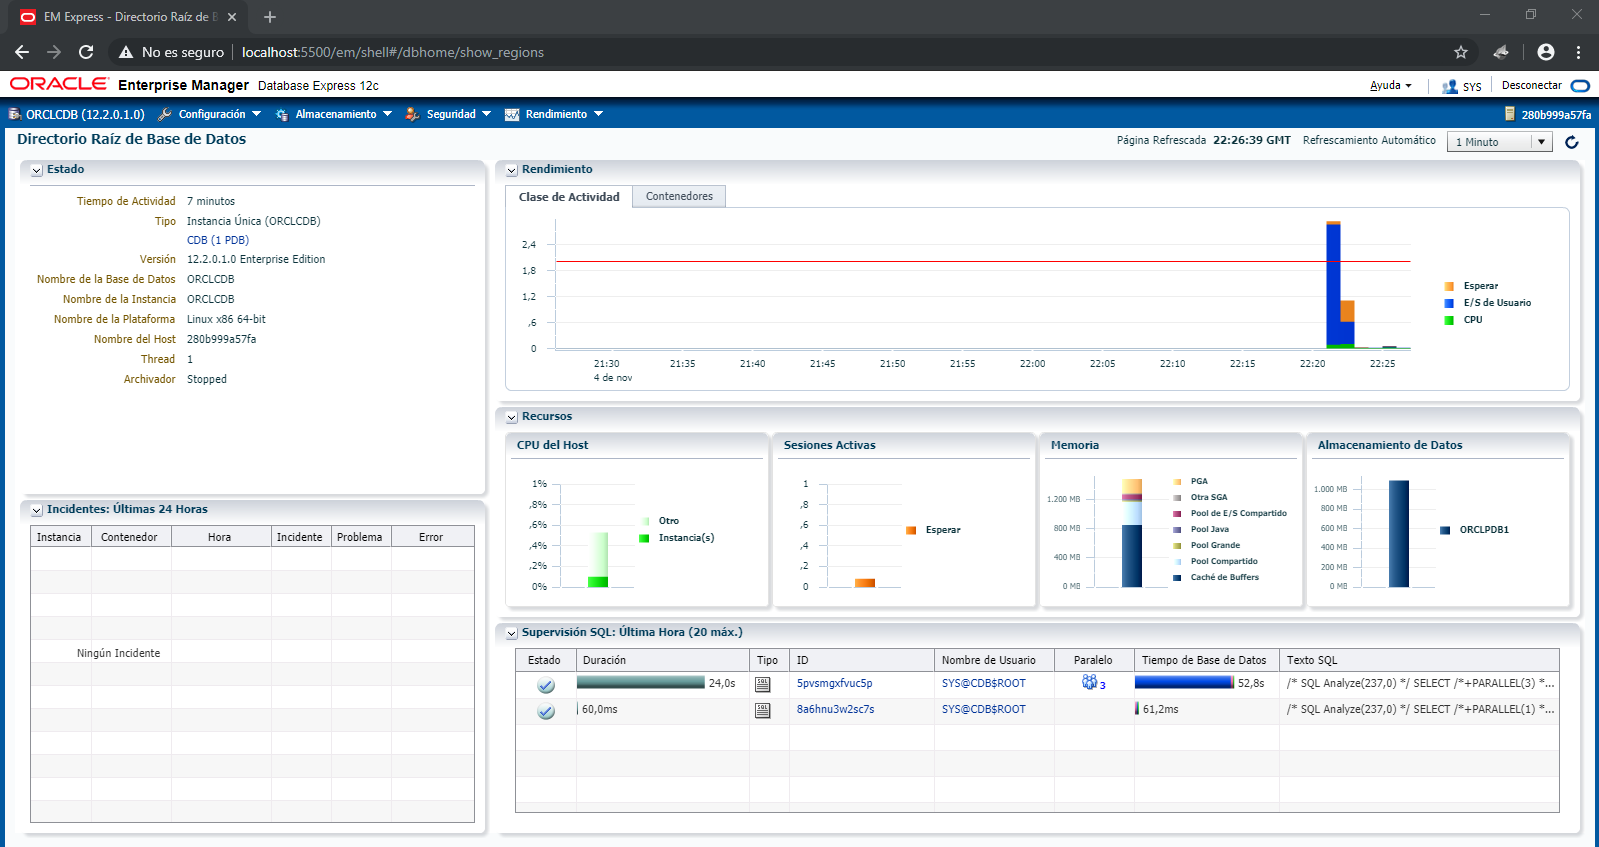
\includegraphics[width=12cm]{./IMAGENES/IMAGEN9} 
		\caption{PANEL DE ORACLE}
	\end{center}
\end{figure}

\begin{figure}[H]
	\begin{center}
		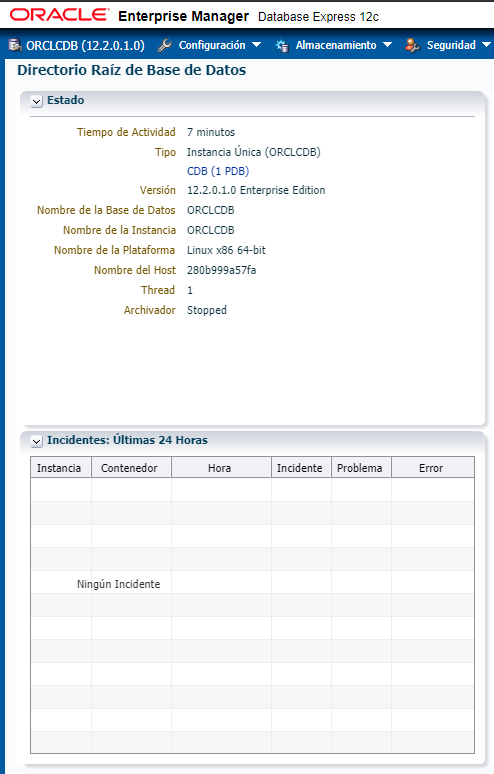
\includegraphics[width=12cm]{./IMAGENES/IMAGEN10} 
		\caption{Directorio raiz de base de datos}
	\end{center}
\end{figure}


\section{ANALISIS E INTERPRETACION DE RESULTADOS }
\begin{itemize}
	\item ¿Qué indican los resultados? \\
	Pudimos realizar exitosamente la conexión de nuestro contenedor a la base de datos
	\item ¿Que se ha encontrado?\\
	Se ha encontrado una forma rapida y eficiente de trabajar con bases de datos sin la necesidad de instalar el servicio.
\end{itemize}

\section{Actividades Encargadas}
\begin{itemize}
	\item¿Con qué comando(s) puedo iniciar y detener una instancia de Oracle, detalle cada uno de los pasos y opciones, utilizando Docker?
 \\
Requiere de estos comandos
	Necesitamos cortar la instancia actual:
	SHUTDOWN IMMEDIATE;
	Iniciar la base de datos en modo MOUNT
	STARTUP MOUNT EXCLUSIVE RESTRICT

	\item ¿Con qué comando(s) puedo iniciar y detener el Listener y el Enterprise manager, detalle cada uno de los pasos y opciones, utilizando Docker?
\\
	lsnrctl start nombreListener arranca el Listener
	lsnrctl stop nombreListener para el Listener
	lsnrctl status muestra información

	emctl start dbconsole arranca el DataBase Control
	emctl stop dbconsole le para
	emctl status dbconsole comprueba el estado actual


	\item . Genere un nuevo contenedor y cree un espacio de tablas con las siguientes características.
Nombre : FINANCIERA:
• DATOS (dbf) : Tamaño Inicial : 50MB, Incremento: 10MB, Ilimitado
• INDICES (dbf) Tamaño Inicial : 100MB, Incremento: 20MB, Maximo: 1GB
• HISTORICO (dbf) Tamaño Inicial : 100MB, Incremento: 50MB, Ilimitado
¿Cuál sería el script SQL que generaría esta base de datos?
	

	CREATE SMALLFILE TABLESPACE "FINANCIERA"
	DATAFILE '//u01/app/oracle/oradata/orcl/DATOS.dbf"
	SIZE 50 MB AUTOEXTEND ON NEXT 10MB MAXSIZE UNLIMITED,

	'//u01/app/oracle/oradata/orcl/indices.dbf"
	SIZE 100MB AUTOEXTEND ON NEXT 20MB MAXSIZE LIMITED 1GB,

	'//u01/app/oracle/oradata/orcl/historico.dbf"
	SIZE 100MB AUTOEXTEND ON NEXT 50MB MAXSIZE UNLIMITED 
	
		
	
\end{itemize}


\section{CONCLUSION}
Los contenedores ayudan a usar bases de datos de forma mas eficiente para poder hacer pruebas o simular ambientes de desarollo o produccion.

\end{document}
